\subsection{UC15 - Selezione prodotto}
\begin{figure}[H]
  \centering
  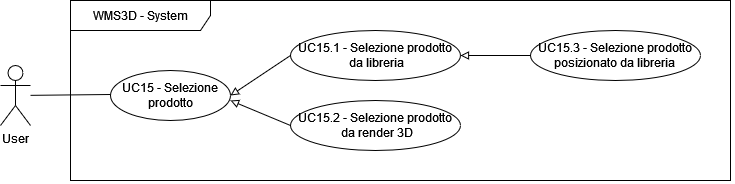
\includegraphics[width=0.8\textwidth]{UC_diagrams_11-20/UC15_sys.drawio.png}
   \caption{Diagramma UML UC15 - Selezione prodotto}
\end{figure}
\begin{itemize}
    \item \textbf{Attori:} User.
    \item \textbf{Pre-condizione:}  L'utente ha creato un prodotto [UC13].
    \item \textbf{Post-condizione:} Il prodotto preso in considerazione dall'utente viene selezionato da libreria o da render 3D.
    \item \textbf{Scenario Principale:} Il prodotto può essere selezionato dalla libreria [UC15.1] e, in tal caso, il prodotto verrà evidenziato in libreria [UC15.1.1] 
    e se il prodotto è posizionato [UC15.3] il prodotto verrà evidenziato anche nel render 3D [UC15.2.1.]. Se invece il prodotto è selezionato dal render 3D [15.2], sicuramente il prodotto è posizionato, e dunque sarà evidenziato su libreria [UC15.1.1] e render 3D [UC15.2.1.].
    \item \textbf{Generalizzazioni:} Sono presenti due generalizzazioni seconda del luogo in cui il prodotto viene selezionato:
    \begin{itemize}
        \item UC15.1 - Selezione prodotto da libreria;
        \item UC15.2 - Selezione prodotto da render 3D;
    \end{itemize}
    \item \textbf{Estensioni:} -
\end{itemize}


\subsubsection{UC15.1 - Selezione prodotto da libreria}
\begin{figure}[H]
  \centering
  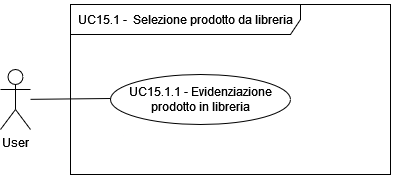
\includegraphics[width=0.8\textwidth]{UC_diagrams_11-20/UC15.1.drawio.png}
   \caption{Diagramma UML UC15.1 - Selezione prodotto da libreria}
\end{figure}
\begin{itemize}
    \item \textbf{Attori:} User.
    \item \textbf{Pre-condizione:}  L'utente ha creato un prodotto [UC13] e lo sta visualizzando nella libreria [UC4.2.1].
    \item \textbf{Post-condizione:} Il prodotto preso in considerazione dall'utente viene selezionato ed evidenziato in libreria.
    \item \textbf{Scenario Principale:} L'utente seleziona il prodotto dalla libreria e il prodotto verrà evidenziato in libreria [UC15.1.1].
    \item \textbf{Generalizzazioni:} È presente una generalizzazione nel caso in cui il prodotto sia posizionato nel magazzino 3D:
    \begin{itemize}
        \item UC15.3 - Selezione prodotto posizionato da libreria.
    \end{itemize}
    \item \textbf{Estensioni:} -
\end{itemize}


\paragraph{UC15.1.1 - Evidenziazione prodotto in libreria}
\begin{itemize}
    \item \textbf{Attori:} User.
    \item \textbf{Pre-condizione:}  L'utente ha selezionato un prodotto.
    \item \textbf{Post-condizione:} Il prodotto preso in considerazione dall'utente viene evidenziato nella libreria.
    \item \textbf{Scenario Principale:} L'utente seleziona il prodotto e questo viene evidenziato sempre nella libreria.
    \item \textbf{Generalizzazioni:} -
    \item \textbf{Estensioni:} -
\end{itemize}


\subsubsection{UC15.2 - Selezione prodotto da render 3D}
\begin{figure}[H]
  \centering
  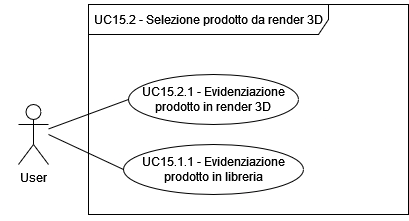
\includegraphics[width=0.8\textwidth]{UC_diagrams_11-20/UC15.2.drawio.png}
   \caption{Diagramma UML UC15.2 - Selezione prodotto da render 3D}
\end{figure}
\begin{itemize}
    \item \textbf{Attori:} User.
    \item \textbf{Pre-condizione:} L'utente ha creato un prodotto [UC13] e lo ha anche posizionato [UC14]. Al momento, lo sta visualizzando nella libreria [UC4.2.1] e nel render 3D [UC3.3].
    \item \textbf{Post-condizione:} Il prodotto preso in considerazione dall'utente viene selezionato dal render 3D ed evidenziato nel render 3D e nella libreria.
    \item \textbf{Scenario Principale:} L'utente seleziona il prodotto dal render 3D e questo verrà evidenziato nel render 3D [UC15.1.1.1] e nella libreria [15.2.1].
    \item \textbf{Generalizzazioni:} -
    \item \textbf{Estensioni:} -
\end{itemize}


\paragraph{UC15.2.1 - Evidenziazione prodotto in render 3D}
\begin{itemize}
    \item \textbf{Attori:} User.
    \item \textbf{Pre-condizione:} L'utente ha selezionato un prodotto posizionato nel render 3D.
    \item \textbf{Post-condizione:} Il prodotto preso in considerazione dall'utente viene evidenziato nel render 3D.
    \item \textbf{Scenario Principale:} L'utente seleziona il prodotto nel render 3D o nella libreria e questo viene evidenziato nel render 3D.
    \item \textbf{Generalizzazioni:} -
    \item \textbf{Estensioni:} -
\end{itemize}


\subsubsection{UC15.3 - Selezione prodotto posizionato da libreria}
\begin{figure}[H]
  \centering
  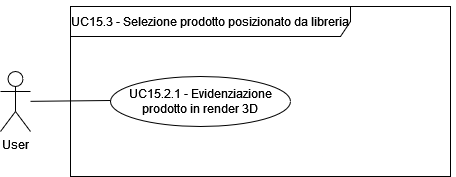
\includegraphics[width=0.8\textwidth]{UC_diagrams_11-20/UC15.3.drawio.png}
   \caption{Diagramma UML UC15.3 - Selezione prodotto posizionato da libreria}
\end{figure}
\begin{itemize}
    \item \textbf{Attori:} User.
    \item \textbf{Pre-condizione:} L'utente ha creato un prodotto [UC13] e lo ha anche posizionato [UC14]. Al momento, lo sta visualizzando nella libreria [UC4.2.1] e nel render 3D [UC3.3].
    \item \textbf{Post-condizione:} Il prodotto preso in considerazione dall'utente viene selezionato dalla libreria ed evidenziato in libreria e nel render 3D.
    \item \textbf{Scenario Principale:} Il prodotto viene selezionato dalla libreria, però questo essendo posizionato, verrà evidenziato sia nella libreria [UC15.1.1] sia nel render 3D [UC15.2.1].
    \item \textbf{Generalizzazioni:} -
    \item \textbf{Estensioni:} -
\end{itemize}

